\section{Evaluation and Conclusion}

\subsection{Strengths}

\begin{frame}{Table 3: Vale Options (VALED)}
  \begin{columns}[T]
    \begin{column}{0.52\textwidth}
      \centering
      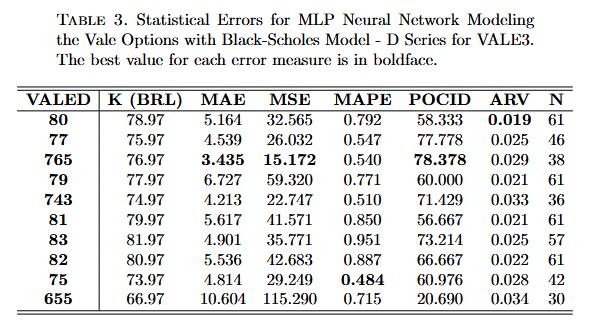
\includegraphics[width=\linewidth]{images/table3.png}
    \end{column}
    \begin{column}{0.44\textwidth}
      \begin{itemize}
        \item Errors vary significantly across contracts
        \item In-the-money options (lower strike) generally show lower errors
        \item Higher errors tend to correspond to less frequently traded contracts
        \item \textbf{Key insight:} NN performance depends on the option's trading activity and moneyness
      \end{itemize}
    \end{column}
  \end{columns}
\end{frame}

\begin{frame}{Figure 3: Model Comparison (VALED)}
  \begin{columns}[T]
    \begin{column}{0.52\textwidth}
      \centering
      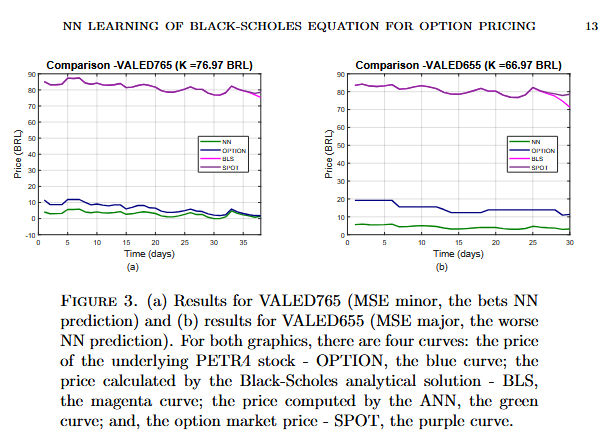
\includegraphics[width=\linewidth]{images/figure3.png}
    \end{column}
    \begin{column}{0.44\textwidth}
      \textbf{Each plot shows three curves:}
      \begin{itemize}
        \item Market price (OPTION)
        \item Black-Scholes solution (BLS)
        \item Neural network output (NN)
      \end{itemize}
      \vspace{0.5em}
      \begin{itemize}
        \item (a) Best NN case: low MSE, NN tracks market closely
        \item (b) Worst NN case: high MSE, NN deviates more noticeably
      \end{itemize}
      \vspace{0.5em}
      \textbf{Key insight:} NN outperforms BLS overall, but accuracy is not uniform across all contracts
    \end{column}
  \end{columns}
\end{frame}

\begin{frame}
\frametitle{Evaluation and Conclusion}
So far, we have seen how the Black-Scholes equation can be derived from financial principles and transformed into a PDE, and how a neural
network can be trained to approximate its solution. \vspace{0.4cm}

In this final section, we will evaluate this approach by briefly discussing its strengths, limitations, and implications for financial modelling.
\end{frame}

\begin{frame}
\frametitle{Strengths of the Neural Network Approach}
Recall the Black-Scholes equation: \[
\frac{\partial V(S,t)}{\partial t}
+ \frac{1}{2}\sigma^2 S^2 \frac{\partial^2 V(S,t)}{\partial S^2}
+ rS \frac{\partial V(S,t)}{\partial S}
- rV(S,t) = 0
\]

\vspace{0.5cm}

We want to approximate the option value $V(S,t)$. By utilising neural networks, we have the following advantages:  
\begin{itemize}
    \item Handles higher dimensions
    \item Applicable Without Closed-Form Solutions
\end{itemize}

\end{frame}

\begin{frame}{Advantage 1: Handles Higher-Dimensional Problems}

In more realistic financial models, the option price may depend on
more than one variable.

\vspace{0.3cm}

For example, an option depending on two assets can be written as
\[
V = V(S_1,S_2,t)
\]

This leads to a larger PDE involving derivatives with respect to
both asset prices.

\vspace{0.3cm}

As the number of variables increases, solving the PDE becomes
more complicated. Neural networks can approximate these
higher-dimensional solutions more easily.

\end{frame}

\begin{frame}{Advantage 2: Applicable Even Without Closed-Form Solution}

Not all options have a simple formula like the standard European call.

\vspace{0.3cm}

For example, an option depending on the average stock price over time:
\[
V = V\Big(S(t), \frac{1}{T}\int_0^T S(t) dt, t\Big)
\]

This makes it difficult to obtain a closed-form solution.

\vspace{0.3cm}

However, the Black--Scholes PDE still applies as it gives a rule that the option price must satisfy, even for these complex cases.

\end{frame}

\subsection{Limitations}

\begin{frame}{Limitation 1: High Computational Cost}

\begin{itemize}
\item Neural networks must be trained using many sampled points from the PDE domain
\item Each training step requires computing derivatives of the network output (PDE residual)
\item This makes training significantly slower than standard finite difference methods for simple PDEs
\item For the Black--Scholes model, closed-form or fast numerical methods are often more efficient
\end{itemize}

\end{frame}

\begin{frame}{Limitation 2: Harder to Interpret}

\begin{itemize}
\item Neural networks are often described as black-box models because the internal decision process is not easily interpretable
\item Unlike analytical Black--Scholes formulas, it is difficult to see how individual inputs (e.g. volatility or strike price) affect the output
\item Model accuracy depends strongly on training data and network design choices
\item This lack of transparency can be a concern in financial settings where interpretability is important
\end{itemize}

\end{frame}

\subsection{Implications for Financial Modelling}

\begin{frame}{Implications for Financial Modelling}

\begin{itemize}
\item Neural networks provide a flexible framework for solving option pricing PDEs
\item They can incorporate market data, potentially capturing effects not reflected in classical models
\item Useful for high-dimensional or complex derivatives where analytical formulas are unavailable
\item Even when closed-form solutions exist, they may not fully match observed market prices
\end{itemize}

\end{frame}

\begin{frame}{Conclusion}

\begin{itemize}
\item The Black--Scholes equation provides a fundamental PDE framework for option pricing in financial mathematics
\item While classical methods rely on analytical solutions or grid-based numerical schemes, these approaches can be limited in complexity and scalability
\item Neural networks offer an alternative approach by directly approximating the PDE solution in a flexible way
\item This makes them particularly useful for high-dimensional problems and financial models
\item However, issues such as computational cost, interpretability, and model validation remain important in practical applications
\end{itemize}

\vspace{0.3cm}

\end{frame}
